\documentclass[12pt, a4paper, hidelinks]{article}

\usepackage[icelandic]{babel}
\usepackage[T1]{fontenc}
\usepackage[utf8]{inputenc}


\usepackage{amsmath, amssymb, amsfonts}
\usepackage{mathtools}

\usepackage{minted}
\renewcommand{\listingscaption}{Forrit}

\usepackage{url}
\usepackage{hyperref}
\usepackage[hang, flushmargin]{footmisc}

\usepackage{xcolor}
\usepackage{tabularx}
\usepackage{graphicx}
\usepackage{booktabs}
\usepackage{enumitem}

\usepackage{fancyhdr}
\pagestyle{fancy}
\fancyhf{}
\fancyhead[L]{Kári Hlynsson}
\fancyhead[C]{TÖL203G HEIMADÆMI \#3}
\fancyhead[R]{\today}
\fancyfoot[C]{\thepage}

\newcommand{\doctitle}{\uppercase{Heimadæmi 3}}
\newcommand{\coursename}{Tölvunarfræði 2}
\newcommand{\coursenum}{TÖL203G}

% ——— Mengjatákn
\newcommand{\N}{\mathbb{N}}
\newcommand{\Z}{\mathbb{Z}}
\newcommand{\Q}{\mathbb{Q}}
\newcommand{\R}{\mathbb{R}}
\newcommand{\C}{\mathbb{C}}

% ——— Vigrar
\renewcommand{\u}{\mathbf{u}}
\renewcommand{\v}{\mathbf{v}}
\renewcommand{\b}{\mathbf{b}}
\newcommand{\w}{\mathbf{w}}
\newcommand{\p}{\mathbf{p}}
\newcommand{\x}{\mathbf{x}}
\newcommand{\y}{\mathbf{y}}
\newcommand{\z}{\mathbf{z}}

\title{}

\begin{document}
\thispagestyle{plain}
\centerline{\bfseries\Large\doctitle}
\medskip
\centerline{\large\coursenum\ \coursename}
\bigskip

\centerline{\large Kári Hlynsson\footnote{Slóð á Github kóða: \url{https://github.com/lvthnn/TOL203G/tree/master/HD3}}}
\bigskip
\centerline{Háskóli Íslands}
\medskip
\centerline{\today}

\bigskip

\noindent
\textbf{\large Verkefni 1} \medskip \\
Breytið \texttt{FourSum.java} í \texttt{FourSumFast.java} á sama hátt og er
gert með \texttt{ThreeSumFast.java}. Skilið kóða fallsins \texttt{count}
(sem texta, ekki skjáskoti) og skjáskoti af keyrslu \texttt{FourSum} og
\texttt{FourSumFast} á gagnaskránni 1Kints.txt. Þá eiga að finnast 13654
ferndir. Athugið að þið þurfið að laga kóðann aðeins, því texttt{FourSum.java}
notar \texttt{long} fylki í stað \texttt{int} fylkis og innlestur gagnanna er aðeins ólíkur.

\medskip
\noindent
\textbf{\large Lausn} \medskip \\
Breytingarnar eru lítillegar og sjást fyrir neðan í forriti \ref{forrit1}.

\begin{listing}[ht!]
    \centering
    \inputminted[firstline=49, lastline=64, linenos]{java}{../src/V1/FourSumFast.java}
    \caption{Fallið \texttt{count} í \texttt{FourSumFast.java}}
    \label{forrit1}
\end{listing}

\noindent
Mynd \ref{mynd1} sýnir keyrslu í skel á \texttt{FourSum.java} og síðan \texttt{FourSumFast.java}.

\newpage
\begin{figure}[ht!]
   \centering
   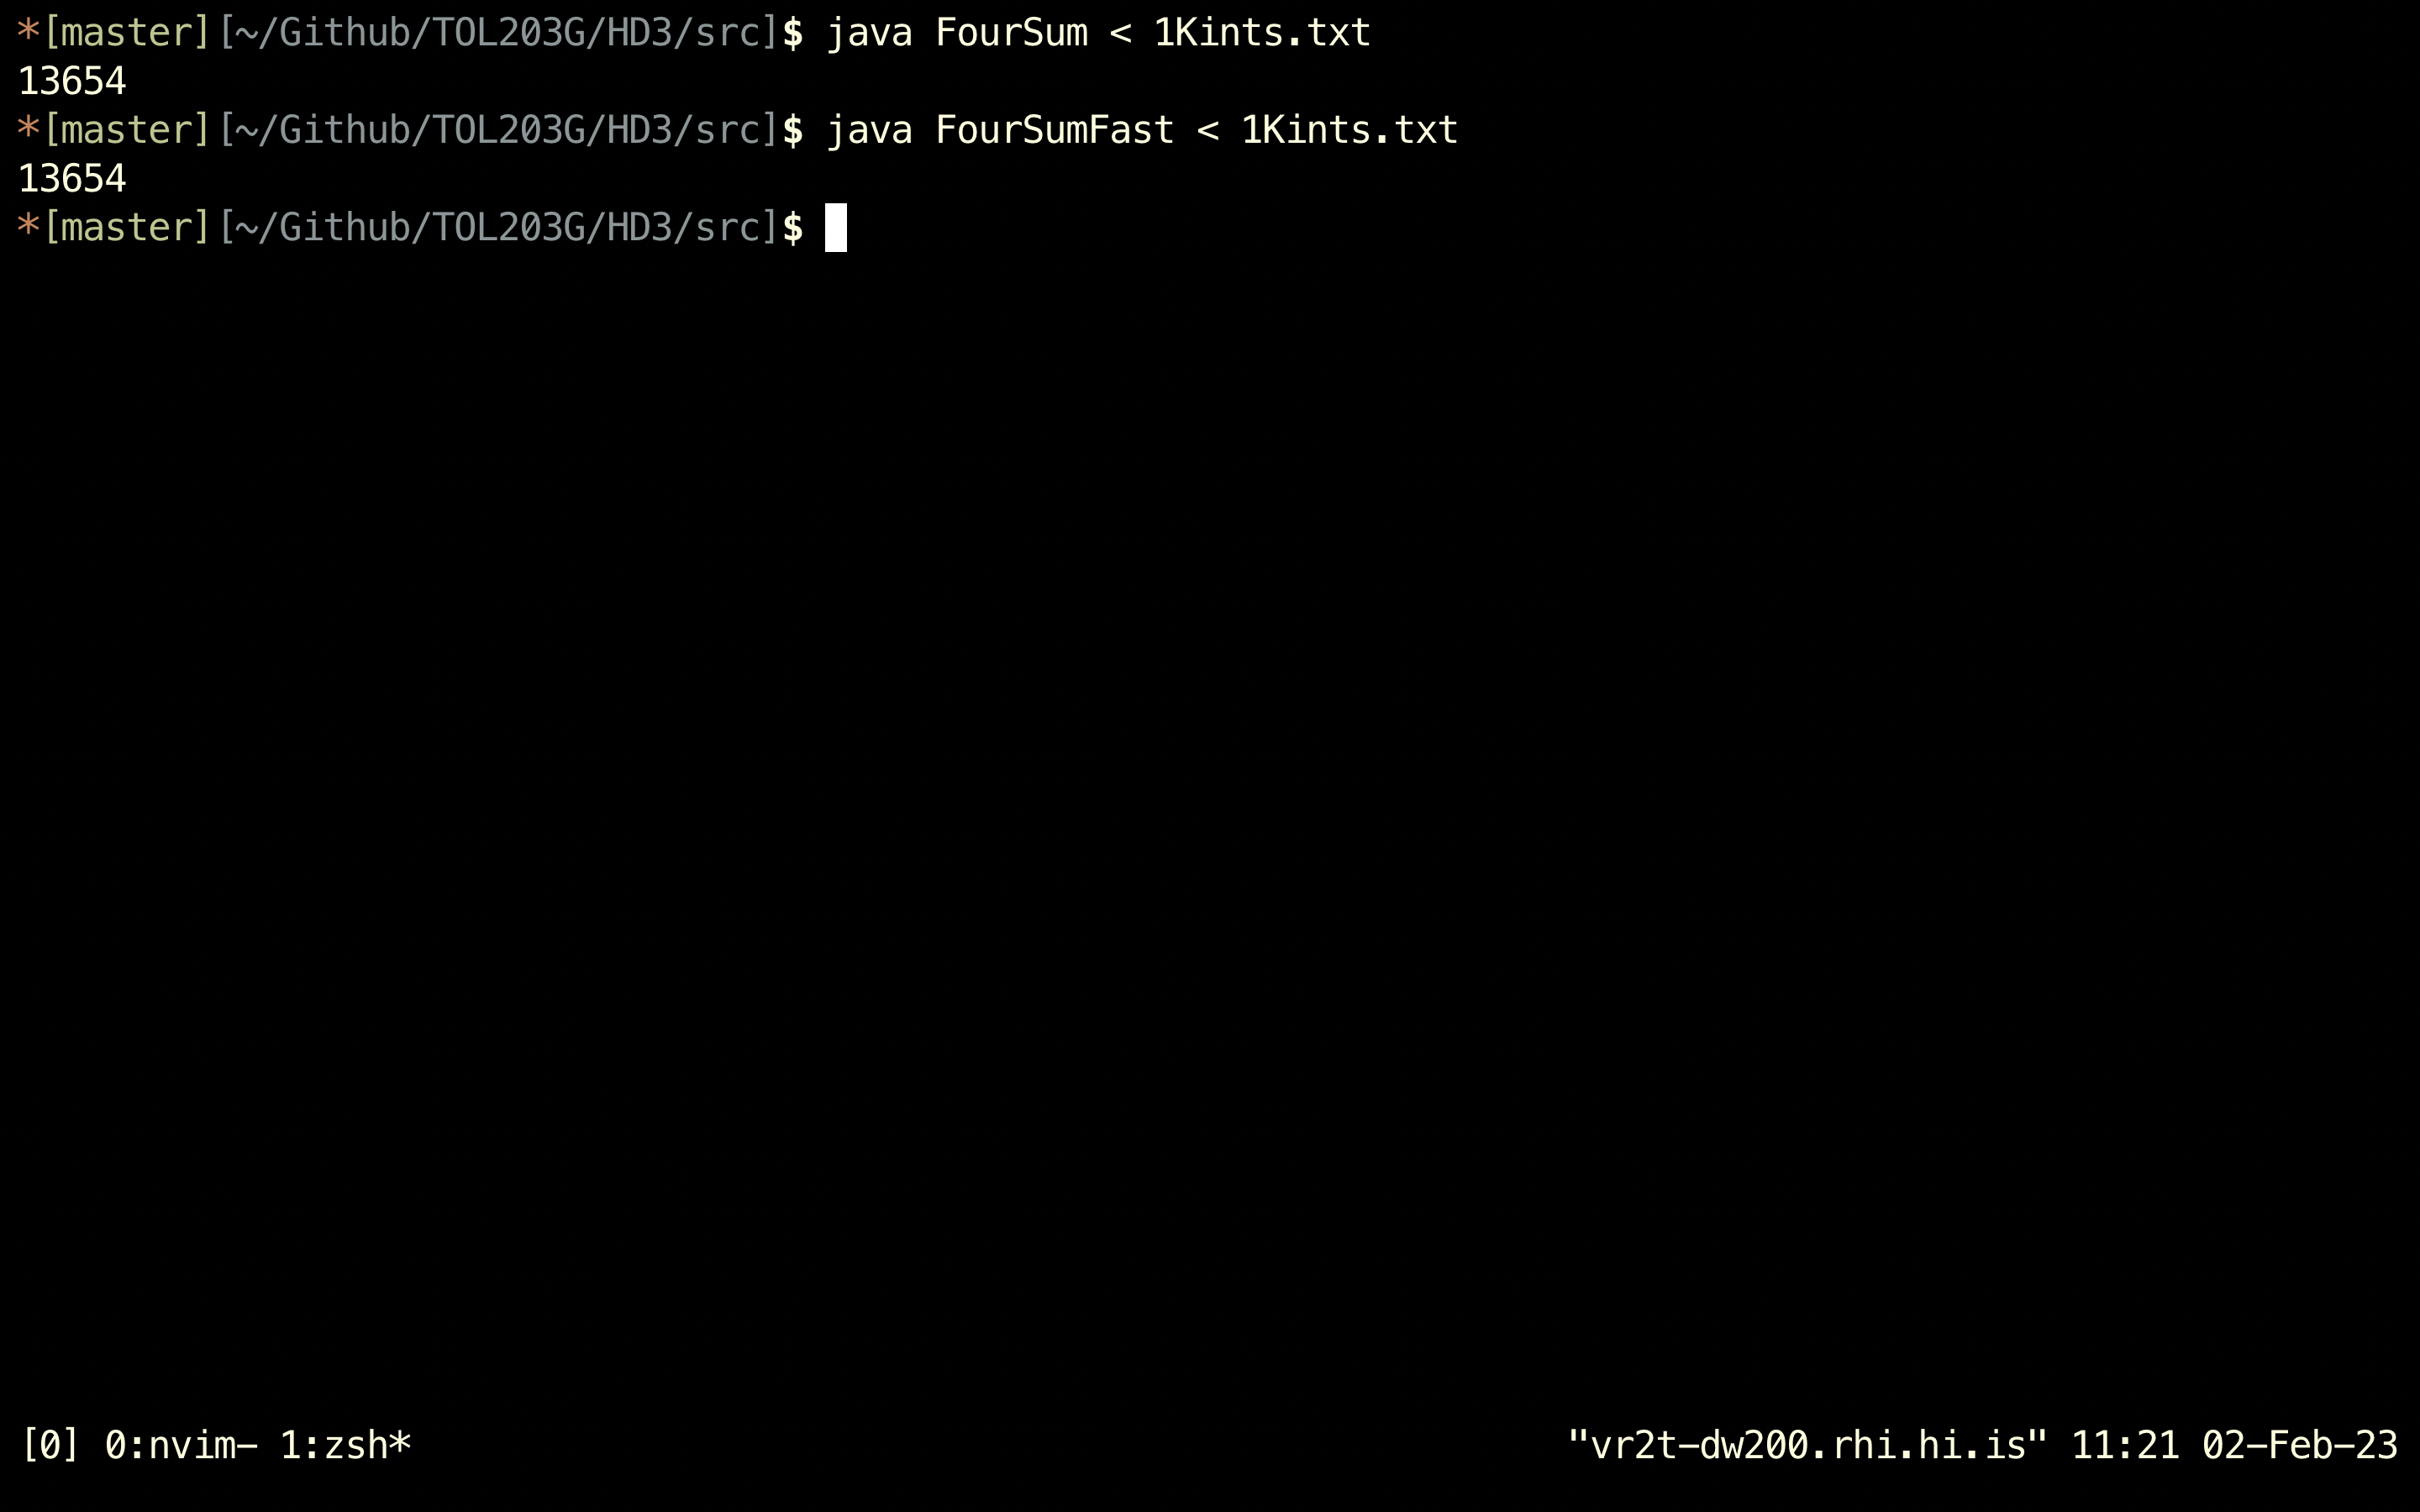
\includegraphics[width=\textwidth]{img/foursum_keyrsla.png} 
   \caption{Keyrsla \texttt{FourSum} og \texttt{FourSumFast} í skel}
   \label{mynd1}
\end{figure}

\noindent
Eins og má sjá fáum við 13654 sem er viðbúinn fjöldi fernda.

\newpage
\noindent
\textbf{\large Verkefni 2} \medskip \\
Framhald af æfingadæminu að ofan.
\begin{enumerate}[label=(\alph*)]
    \item Finnið raunhæf neðri mörk á vaxtarhraða keyrslutíma reiknirits sem leysir þetta verkefni, þ.e. hversu margar
    aðgerðir þurfa öll reiknirit að nota til þess að leysa þetta verkefni (sem fall af $N$)? Rökstyðjið svarið í nokkrum
    orðum.

    \item Það er hægt að leysa verkefnið á mun hraðvirkar hátt en gert var í æfingadæminu, með því að nýta sér fyrri útreikninga
    í $B$. Hugmyndin er þið eruð að reikna út \texttt{B[i,j]} þá eruð þið nýbúin að reikna út \texttt{B[i, j-1]}. Er ekki hægt að
    nota það gildi? Útfærið þetta reiknirit í Java og keyrið það fyrir sömu gildi á $N$ og gert var í æfingadæminu. Hver er vaxtarhraði
    þessa nýja reiknirits? Skilið kóðanum (sem texta, ekki skjáskoti) og svarinu.
\end{enumerate}

\medskip
\noindent
\textbf{\large Lausn} \medskip \\
\textbf{Hluti (a)} \medskip \\
Látum $\sigma(i, j) \coloneqq \sum_{k = i}^j a_k$.\footnote{Við notum hér bilið $1, \ldots, N$ í stað $0, \ldots, N-1$
eins og venja er fyrir í stærðfræðilegum rithætti fyrir runur. Þá er inntakið okkar heiltöluruna á forminu $a_1, \ldots, a_N$.} Við getum sett upp töflu sem sýnir hvernig
fylkið $B$ lítur út fyrir gefna inntaksstærð $N$:

\renewcommand{\arraystretch}{1.25}
\begin{table}[ht!]
    \centering
    \begin{tabular}{ccccc}
        \toprule
        $\downarrow$ i $\rightarrow$ j &  1 & 2 & $\cdots$ & N \\
        \midrule
        1        & $\sigma(1, 1)$ &— & $\cdots$ & — \\
        2        & $\sigma(2, 1)$ &$\sigma(2, 2)$ & $\cdots$ & — \\
        $\vdots$ & $\vdots$ & $\vdots$ & $\ddots$ & $\vdots$ \\
        $N$ & $\sigma(N, 1)$ & $\sigma(N, 2)$ & $\cdots$ & $\sigma(N, N)$ \\ 
        \bottomrule
    \end{tabular}
    \caption{Útlit fylkisins $B$.}
\end{table}

\noindent
Við miðum almenna kostanaðarlíkanið út frá fjölda fallakalla á $\sigma(i, j)$. Við sjáum
að heildafjöldi kalla er $1 + 2 + \cdots + N$ svo við fáum
\[
    T(N) = 1 + 2 + \cdots + N = \frac{N(N + 1)}{2} \sim \frac 12 N^2
\]
m.ö.o. er $T(N) \sim \Omega(N^2)$.

\newpage
\noindent
\textbf{Hluti (b)} \medskip \\
Við skulum hefja umfjöllunina á upprunalega fallinu. Ef við útfærum sauðakóðann
sem er gefinn í æfingadæminu í Java fáum við eftirfarandi forritsbút:

\begin{listing}[ht!]
    \centering
    \inputminted[firstline=13, lastline=22, linenos]{java}{../src/V2/ArraySum.java}
    \caption{Fallið \texttt{arraysum} (hægari útfærsla)}
    \label{forrit2}
\end{listing}

\noindent
Í þessari aðferð útfærum við hlutsummufallið $\sigma(i, j)$ með því að ítra í gegnum bilið
með $i \leq k \leq j$, sækja gildið $a_k$ hverju sinni og leggja við $b_{ij}$. Þessi aðferð
er línuleg, þ.e. kostnaður hennar er $N$ á heildina litið og því er tímaflækja þessa forritsbúts
$T(n) \sim \mathcal O(N^3)$.

Hin útfærslan er mun hraðvirkari. Hún gengur þannig fyrir sig að við ítrum sem áður í gegnum fylkið.
Ef við erum í hornalínustaki er það fyrsta stakið sem leggur eitthvað til summunnar og því setjum við
einfaldlega $B_{ij} = A_i$ ef $i = j$.\footnote{Þetta getur allt að eins verið $A_j$ því $A_i = A_j$ því $i = j$.} 
Ef svo er ekki þá setjum við $B_{ij} = B_{i, j-1} + A_j$ því við höfum þegar reiknað $B_{i, j-1}$. Forritsbúturinn er gefinn fyrir neðan:

\begin{listing}[ht!]
    \centering 
    \inputminted[firstline=31, lastline=39, linenos]{java}{../src/V2/ArraySum.java}
    \caption{Fallið \texttt{arraysum\_fast} (hraðari útfærsla)}
    \label{forrit3}
\end{listing}

\begin{figure}[ht!]
    \centering
    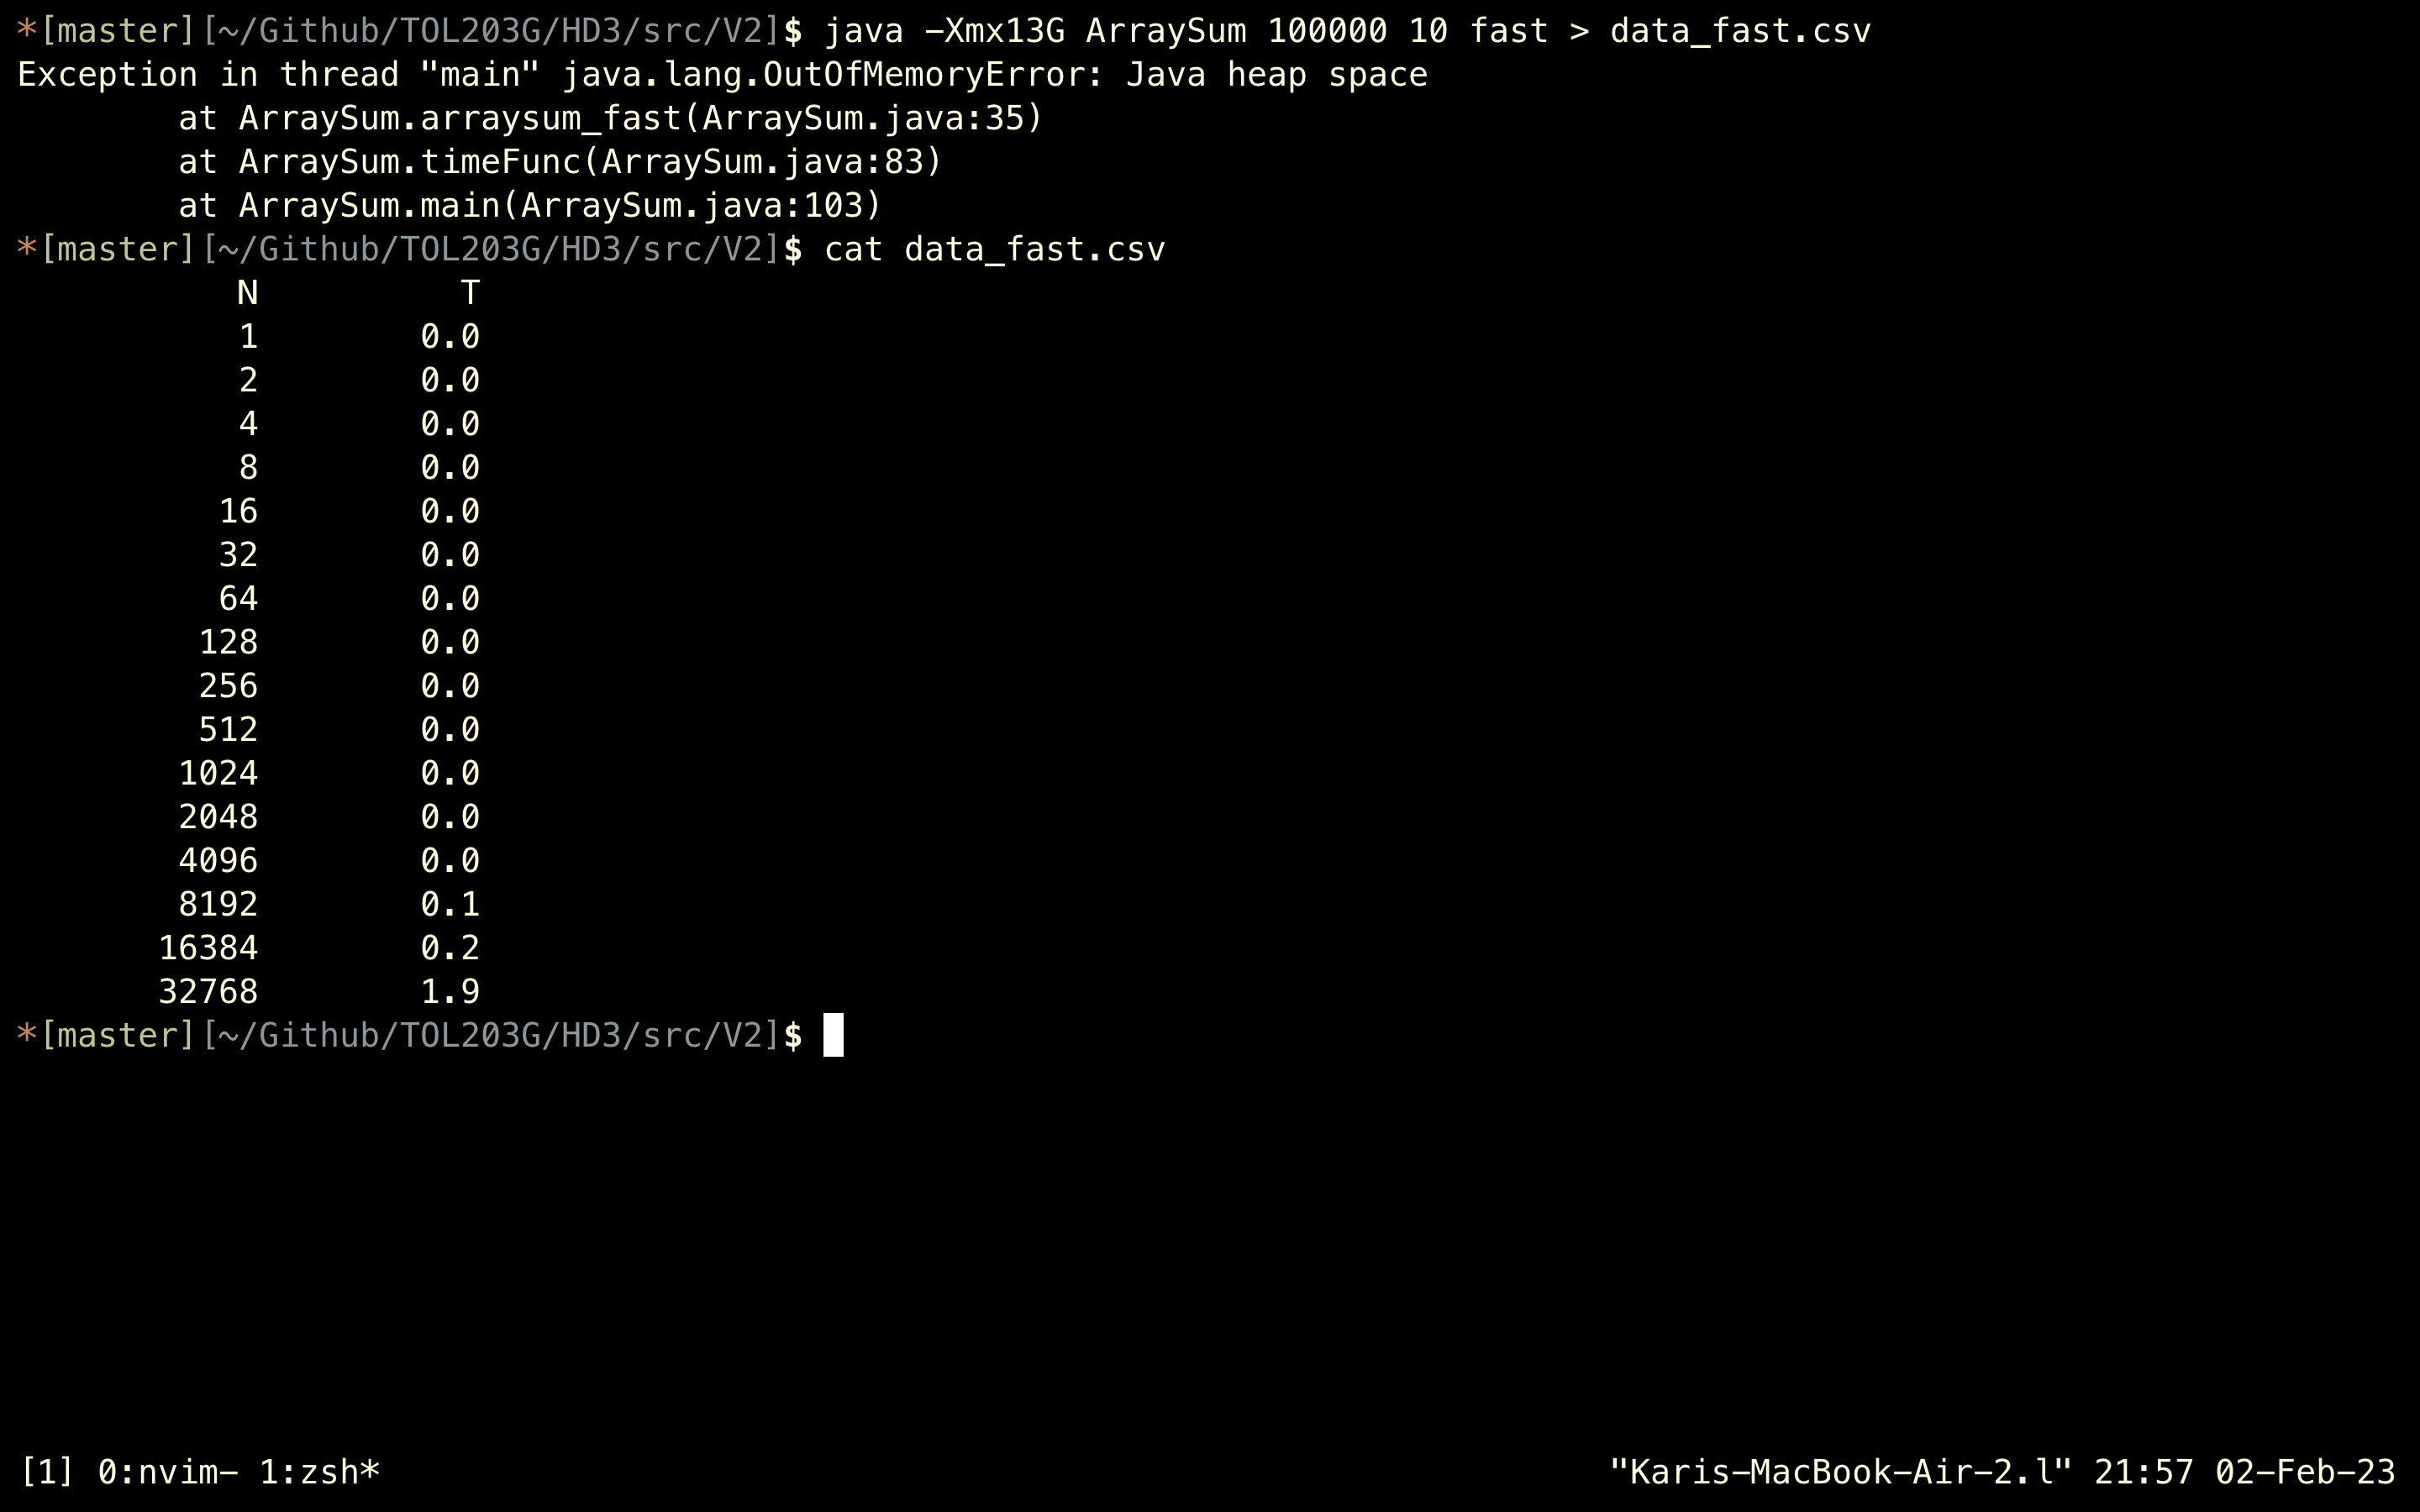
\includegraphics[width=\textwidth]{img/arraysum_keyrsla.png}
    \caption{Keyrsla á \texttt{ArraySum.java} og söfnun gagna}
    \label{mynd2}
\end{figure}

\noindent
Útfærslan í forriti \ref{forrit3} tryggir $\sigma(i, j) \sim \mathcal O(1)$ þ.e. summuaðgerðin er fasti hverju sinni svo við
búumst við því að $T(N) \sim \mathcal O(N^2)$ fyrir þessa útfærslu. Við göngum úr skugga um þetta með mælingum.

Látum $T_s(N)$ tákna tímaflækju meintu hægari útfærslunnar en $T_f(N)$ tákna meintu
hraðari útfærsluna. Við spáðum fyrir að $T_s(N) \sim \mathcal O(N^3)$ og að $T_f(N) \sim \mathcal O(N^2)$.
Við keyrum notendaforritið í skel og beinum staðalúttakinu í csv skrá til frekari úrvinnslu, eins og mynd fyrir neðan sýnir.

Mynd \ref{mynd2} sýnir keyrsluna á \texttt{ArraySum.java}. Stillingin \texttt{-Xmx13G} til að gefa forritinu $13$ GB
til keyrslu en þá getum við fengið aðeins meiri gögn. Hið sama var endurtekið á nýjan leik fyrir hægari útfærsluna.
Línulegt aðhvarf var framkvæmt í R þar sem við fengum hallatölu $2.292 \approx 2$ fyrir \texttt{arraysum_fast} en $2.832 \approx 3$
fyrir \texttt{arraysum} sem ber einmitt saman við tilgátu okkar um tímaflækju reikniritanna.

\begin{figure}[ht!]
    \centering
    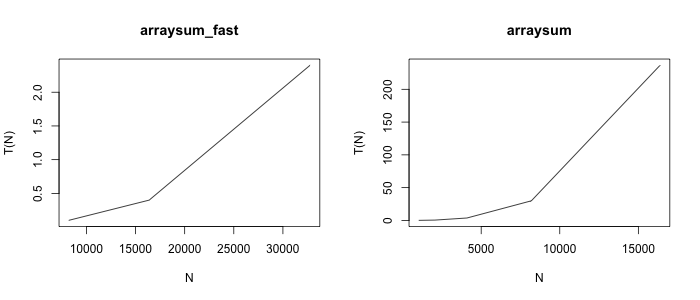
\includegraphics[width=\textwidth]{img/speed_comparison_nonlog.png}
\end{figure}


\newpage
\noindent
\textbf{\large Verkefni 3} \medskip \\
Tiltekið hótel hefur $N$ herbergi, sem eru í röð á löngum gangi. Herbergi $0$ er næst móttökunni, en herbergi $N-1$ er lengst í burtu.
Öll herbergin frá $0$ til $F-1$, en herbergi $F$ til $N-1$ eru laus. Við viljum sjálf vera í herbergi $F$, en við vitum ekki gildið á $F$
(aðeins að $F < N$). Til þess að finna fyrsta lausa herbergið getum við aðeins kannað eitt herbergi í einu með því að banka á hurðina og kíkja
inn. Við viljum lágmarka fjölda skipta sem við bönkum á hurðir í versta tilfelli.

\begin{enumerate}[label=(\alph*)]
    \item Hver er versta tilfellis tími (sem fall af $N$) á reikniriti sem byrjar á herbergi $0$ og rekur sig út eftir ganginum þar til fyrsta
    lausa herbergið er fundið?
    \item Lýsið reikniriti sem notar í versta falli $\log N$ tíma til að finna fyrsta lausa herbergið.
    \item Ef $N$ er mikið stærra en $F$, þá er hægt að gera betur og nota aðeins $\sim 2 \log F$ tíma til þess að finna fyrsta lausa herbergið.
    Lýsið þessari aðferð og rökstyðjið vaxtarhraða hennar.
\end{enumerate}

\medskip
\noindent
\textbf{\large Lausn} \medskip \\
\textbf{Hluti (a)} \medskip \\
Ef við gefum okkur að aðferðin er að fara hurð eftir hurð eftir ganginum fæst versta tilfellið þegar
$F = N-1$. Þá er tímaflækjan nokkurn veginn $\sim N$.

\medskip
\noindent
\textbf{Hluti (b)} \medskip \\
Til þess að útfæra þetta notum við afbrigði af binary search.

\end{document}